\chapter{テーブル全体への作用}


\section{UPDATEの作用}

テーブル全体に対するUPDATEの考え方を説明します。
UPDATEは、カーソルなどを使わずに、テーブルを更新します。条件に合致するレコードを変更することで、テーブルを変化させます。、

テーブルに作用するUPDATEとは、どのような性質を持つものなのでしょうか。

\subsection{全てのレコードをUPDATE}
全てのレコードを一度にアップデートするのは、SQLの得意とするところです。UPDATEを1行書けば、それで全てのレコードを更新することができます。

たとえば、全てのユーザに詫び石を100個配る、というソーシャルゲームでありがちなシチュエイションを考えてみましょう。\footnote{石というのは、スマートフォンなどのソーシャルゲームで、有償のサービスを受けるために購入する、ゲーム内通貨の俗称です。宝石をトークンのイメージとすることが多いため、石、と呼ばれます。この石は、サービスにトラブルがあった際に、ユーザに無償配布されることがあります。それを俗に詫び石とよんでいます}

usersテーブルの整数型フィールドstoneを石の数とします。全てのユーザに石を追加するクエリは、\ref{sql:update}のように書くことができます。
一般的な手続き型言語のように、特定のレコードを指定するループ処理は必要ありません。

\begin{lstlisting}[caption=全体に作用するupdate,label=sql+update]
UPDATE users SET stone - stone + 100 WHERE 1;
\end{lstlisting}

厳密には、トランザクションへの考慮が入っていなかったりしますが、ここではこの形で説明をします。このクエリは、usersテーブルのレコードで該当するレコードのフィールドstoneを、元の数に100をくわえた値でアップデートする、という意味です。レコードを選択するときの条件に1がはいっているので、常に真であり、その結果、全てのレコードが対象となります。


\subsection{UPDATEの考え方}

前著の「ゆるいSQL]では、SELECTは、テーブルからテーブルへの写像、つまり、空間から空間への写像という説明をしました。では、UPDATEは、どのように考えれば良いのでしょうか。

UPDATEも、テーブルとテーブルの間の写像であることには変わりありません。つまり、二つの集合の間の写像です。ですが、見た目として、同じテーブルの間でおこなわれているため、混乱します。

このことを考えるために、状態という概念をもちこんでみましょう。n番目の状態というのを、元のテーブルから、n回なんらかのUPDATEを行ったときのテーブルの内容と考えます。CRETEしたばかりのテーブルは、0番目の状態であるとします。
これは、UPDATEを行うと、n-1番目のテーブル、という状態から、n番目の状態へ移行すると考えることができます。

\begin{figure}[htbp]
  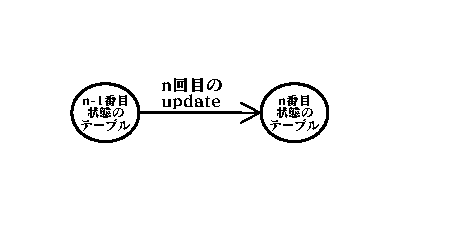
\includegraphics[width=8cm,pagebox=cropbox]{draw/update1.pdf}
  \caption{UPDATEと状態遷移}
  \label{fig:change}
\end{figure}

このような概念を、状態遷移といいます。UPDATEの解釈に状態遷移の概念を持ち込んだとき、UPDATEとは、n-1番目の状態から、n番目の状態への場外戦意であり、写像関係である、と考えることができます。

ですが、RDBMSのテーブルは、そのテーブルだけで過去の状態を保存することができません。
\footnote{どうしても保存したい時は、保存したいテーブルの構造にシーケンスを付加した別のテーブルを作って、UPDATEをする前に、毎回コピーを格納していく、というようなやりかたを取れば可能です。}
そのため、n回目のUPDATEを行った後は、n番目の状態のみが見えて、アクセスできる状態であると考えることができます。

あるいは、0番目からはじまる各状態のテーブルがおくから繋がっていて、一番手前にあるのがn番目の状態であり、見ている方向からはそれしか見えない、という考え方もできます。

\subsection{UPDATEはどういう操作か}

結局のところ、UPDATEとは、テーブルにどのように作用する操作なのでしょうか。
ここまでで、UPDATEは、テーブルの状態を変化させて、次の状態に遷移させる操作として説明しました。

ここまで明記していませんでしたが、UPDATEでは、n-1番目状態と、UPDATEが作用した結果である、n状態との間で、その要素の数は変化しません。また、n-1番目の状態のテーブルの構造と、n番目の状態のテーブルの構造も変化しません。

テーブルを多次元の直交座標空間と見なして考えてみましょう。\footnote{この考えは、前著の「ゆるいSQL]で展開したものです。}フィールドは、直交する座標軸に相当します。
その中に、0個以上のレコードがあります。レコードがその空間の中のどこにあるかは、各フィールドの値がを座標の値として考えることで現されます。

このように考えたとき、n-1番目の状態で、k個のレコードが、テーブルが現す空間のどこかにばらまかれているというイメージとなるでしょう。

UPDATEは、その中の0個以上のイメージを空間内の別の場所に動かし、その結果をn番目の状態と見なす、という操作となります。

\begin{figure}[htbp]
  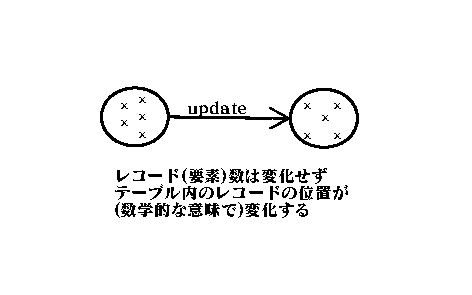
\includegraphics[width=8cm,pagebox=cropbox]{draw/update2.pdf}
  \caption{UPDATEによる変化}
  \label{fig:move}
\end{figure}


UPDATEでは、その操作の前後で、空間構造、つまり、フィールドの種類や属性は変化しません。また、要素の数、つまり、レコードの数も変化しません。

\section{テーブルへの操作とトランザクション}

最初に挙げたUPDATEの例は、実際の環境では失敗することがあります。
ノイマン型のコンピュータアーキテクチャでRDBのエンジンを実行するとき、アセンブラのレベルでは実時間を使ったループで処理されているためです。
そのため、そのループ中に割り込みやメモリ、ディスクのトラブルが生じれば、UPDTEの処理が失敗します。

これは、UPDATEという処理が、実際には多数の小さな処理に分割されて実行されているためです。ですが、RDBとしては、UPDATEという処理は、分割できない単一のものとして扱いたい、という要望があります。

このように、RDBの立場で、分割されない処理という概念を、アトミックとよんでいます。
これは、原始のアトミックと同じ意味です。
そして、RDBMSには、アトミックと、アトミックを担保するトランザクションという二つの概念があります。

トランザクションは、現実の世界でアトミックを保証する仕組みです。これは、アトミックに行われなければならない操作が完結したときのみ、その操作を有効にします。先程のUPDATEの例でいけば、n-1番目の状態からn番目の状態に遷移するのに必要な操作が全て完了したときだけ、n番目の状態を有効にします。

数学的な意味だけで考えれば、UPDATEによるテーブルへの操作は、レコードの情報の変化、要素の移動という結果が出ます。
それなら、なぜ、トランザクションやアトミックという概念が出るのでしょうか。、

\subsection{アトミック}
アトミックという言葉には、それ以上分割できない、という意味があります。アトミックな処理とは、中断されずに完了されるべき処理、ということです。

数学的な意味のUPDATEとは、あるテーブルという空間の、0個以上のレコードという要素を選択して、空間の中での位置を変化させるという操作です。

ですが、実際のコンピュータの処理では、数学的な意味通りの動きはできません。RDBMSのエンジンの中では、ループ的な処理が行われます。それは、レコードが記載されたストレージやメモリを読んで、WHEREに記述された条件に一致するレコードであれば、SETに書かれた内容でレコードの中身を更新する、というものです。

そのため、UPDATEの対象となるレコードが1個以上あり、そのレコードに変更されるフィールドが1個以上存在すれば、実時間を使って処理を行う必要があります。
そして、コンピュータの実時間処理というのは、常に、中断される可能性があります。
つまり、現実の世界ではアトミックに処理を完結できる保証はありません。

その条件下でアトミックに処理を完結させるには、どのようにすれば良いのでしょうか。
それは、アトミックな処理、というのを、全部終わらせなければ完了にならない処理として定義し、それが完了したことを確認した場合のみ、結果に反映するやり方です。

また、アトミックという概念は、ひとつのUPDATEだけに限りません。
複数のSQL文で写像関係を定義するとき、それは関数となります。
そして、その関数によるマッピングが、アトミックに行われなければならないという場面もあります。
このように、複数のSQL処理全体に対して、アトミック性を保証したい、という場合もあります。

次に説明するトランザクションの概念は、多くの場合、複数のSQLによる一連の処理にアトミック性を担保するために用いられます。

\subsection{トランザクション}

RDBMSの一つ一つの操作は、本質的にアトミックであるべきです。ですが、現実には、中断の可能性がある計算機上の処理として行われています。

そんな現実世界でアトミックであることを実現するには、処理が完了した場合のみ、結果に反映する、という方法を採ります。そして、処理が途中で失敗した場合は、そこまでの成果を全て捨て、操作自体を行う前の状態に戻します。

この、完了したときだけ結果に反映する、完了しなければ操作する前に戻す、という考え方がトランザクションです。

\subsection{トランザクションの範囲}

この考え方を拡張すると、複数のSQLによる操作をマクロと見て、そのマクロ操作に対してトランザクションを適用する、という考えになります。

実際のSQLでは、アトミックにしたい一連の操作をはじめるときに、トランザクションであるという宣言をします。MySQLの場合は、START TRANSACTIONというステートメントになります。
トランザクションを宣言した以降の操作は、結果の反映を指示するコマンドが投入されるまで、実際のデータベースには反映されません。

また、なかったことにするコマンドを投入すれば、トランザクションの宣言以降の操作は破棄され、操作されていたテーブルは、トランザクションを宣言する直前の状態に戻ります。

MySQLやMariaDBでは、START TRANSACTIONで、トランザクションの開始を宣言します。そして、COMMITで、トランザクション宣言以降の操作が全て成功したものと見なして、それまでの操作を全て反映します。

\begin{lstlisting}[caption=コミットで完結するトランザクション,label=sql:commit]
START TRANSACTION

# この中のSQLによる操作はコミットまで反映されない

# COMMITでここまでの操作が反映される
COMMIT
\end{lstlisting}

逆に、ROLLBACKを使用すると、それまでの処理が全て破棄されて、トランザクションを宣言する前の状態に戻ります。

\begin{lstlisting}[caption=ロールバックで終わる場合,label=sql:rollback]
# ROLLBACKするとこの時点の状態に戻る
START TRANSACTION

# この中のSQLによる操作はROLLBACKで破棄される

ROLLBACK
\end{lstlisting}

\subsection{トランザクションロック}
トランザクションを宣言された以降の操作は、完結するまで反映されません。
この操作を完結させるためには、操作途中にデータに矛盾が発生してはならない、ということでもあります。
この矛盾は、トランザクションが一連の操作を行っている間に、そのトランザクション以外のクエリでテーブルの内容が操作された場合に発生する可能性があります。

たとえば、全てのレコードへのUPDATEを行っている最中に別のクエリがレコードの追加を行った場合、その追加されたレコードはUPDATEされるべきかどうか、そういう問題が生じ、それは元の操作のアトミック性を破壊したことになります。

それを防止するためには、トランザクションの外からのテーブルへのアクセスをロックします。具体的には、読み出しはトランザクション宣言直前の、まだ操作されていない状態のテーブルを参照することになります。
また、書き込みに関しては、トランザクションが完了するまで、トランザクション内で操作されたテーブルは操作がロックされます。つまり、トランザクションの外のクエリは、結果にカカウォーズ、トランザクションが週リュオウするまでまたされます。

ここまで説明したように、トランザクションロックがあるため、トランザクションは、COMMITもしくはROLLBACKで完結する必要があります。そのため、もしトランザクション中にエラーが発生した場合は、例外処理としてROLLBACKを実行するようにコードを記述します。

クエリ\ref{sql:transaction}は、トランザクション中のSQLで何らかのエラーが発生した場合、それを例外処理で受けて、ROLLBACKして終了する例です。実際の処理では、SQLを喚びだしたプロセス側にもROLLBACKを伝えて例外処理をする必要があるのですが、その部分は省略しています。

\begin{lstlisting}[caption=トランザクションロックとエラー処理,label=sql:transaction]
# トランザクションの外からはこの時点のテーブルが見える
START TRANSACTION

# トランザクション中にエラー(例外)発生時点でROLLBACKしてトランザクション終了
DECLARE EXIT HANDLER FOR SQLEXCEPTION ROLLBACK

# トランザクション処理

# ここまでの処理が成功したら結果を反映
COMMIT

# この時点でトランザクションロックが解消される

\end{lstlisting}